\documentclass[
    %draft,
    %handout,
    % font size
    11pt,%
    % layout: 16:9
    aspectratio=169,%
    % layout: 4:3
    %aspectratio=43,%
]{beamer}
\usepackage[ampersand]{easylist}
\usepackage{fontspec}
\usepackage{polyglossia} % XeLaTex replacement for babel
% Assumes English as the primary and German as the secondary language
\setmainlanguage{english}
\setotherlanguage[spelling=new,latesthyphen=true]{german}
\usetheme[
    %sectionpage=simple,% looks like standout/plain
    sectionpage=progressbar,
    progressbar=frametitle,%
    block=fill,%
]{metropolis}
%%%%%%%%%%%%%%%%%%%%%%%%%%%%%
%  V A R I A B L E S -- Begin

% AUTHOR
\newcommand{\docAuthorName}{Dominik}
\newcommand{\docAuthorSurname}{Gedon}
\newcommand{\docAuthor}{\docAuthorName{} \docAuthorSurname{}}
% TITLE / SUBTITLE
\newcommand{\docTitle}{The Root of All Evil}
\newcommand{\docSubTitle}{How Dangerous is Rooting Your Android?}
% DATE
\newcommand{\docDate}{\today}
% INSTITUTE
\newcommand{\docInstituteGroup}{Security Research Group}
\newcommand{\docInstituteDepartment}{Department of Computer Science}
% Naming convention for English publications: https://www.fau.de/files/2013/09/Verwendung_Uniname_EN.pdf
\newcommand{\docInstituteUniversity}{Friedrich-Alexander University Erlangen-Nürnberg (FAU)}
\newcommand{\docInstitute}{\docInstituteGroup{}\\\docInstituteDepartment{} \\\docInstituteUniversity{}}
% HASHTAG
\newcommand{\docHashtag}{\#faui1}

%  V A R I A B L E S -- End
%%%%%%%%%%%%%%%%%%%%%%%%%%%%%
% Modify Metropolis theme
%%%%%%%%%%%%%%%%%%%%%
%  C O L O R -- Begin

\definecolor{33c3Teal}{RGB}{0,156,139}
\definecolor{33c3Purple}{RGB}{91,68,151}
\definecolor{33c3Yellow}{RGB}{255,244,95}
\definecolor{33c3Salmon}{RGB}{229,76,139}
\definecolor{33c3Blue}{RGB}{0,113,193}
\definecolor{33c3Gray}{RGB}{70,71,73}
\definecolor{33c3Green}{RGB}{141,193,35}
\definecolor{33c3Red}{RGB}{255,38,60}
\definecolor{33c3White}{RGB}{255,255,255}

\setbeamercolor{normal text}{%
    fg=black,
    bg=black!2
}

\setbeamertemplate{title separator}{
	\begin{tikzpicture}
	\draw[fg, fill=fg] (0,0) rectangle (\textwidth, 0.5pt);
	\end{tikzpicture}%
	\par%
}

\setbeamercolor{frametitle}{%
    use=palette primary,
    parent=palette primary,
    bg=33c3Gray
}
\setbeamercolor{alerted text}{%
  fg=33c3Teal%
}
\setbeamercolor{example text}{%
  fg=33c3Blue%
}

%  C O L O R -- End
%%%%%%%%%%%%%%%%%%%%%

%%%%%%%%%%%%%%%%%%%%%%%%%%%%%%%%%%%%%%%%%%%%%%
%  M I S C  M O D I F I C A T I O N S -- Begin

% Make the footline gray
\setbeamercolor{footline}{fg=33c3Gray}

\setbeamercolor{section page}{bg=33c3Gray}

% Display the hashtag in the footer
%\setbeamertemplate{frame footer}{\docHashtag{}}

% Color `standout` (aka `plain`)
%\providebool{metropolis@standout}
%\define@key{beamerframe}{standout}[true]{%
%    \booltrue{metropolis@standout}
%    \begingroup
%        \setkeys{beamerframe}{c}
%        %\setkeys{beamerframe}{noframenumbering}
%        \ifbeamercolorempty[bg]{palette primary}{
%            \setbeamercolor{background canvas}{
%                use=palette primary,
%                bg=-palette primary.fg
%            }
%        }{
%            \setbeamercolor{background canvas}{
%                use=palette primary,
%                bg=33c3Gray
%            }
%        }
%    \setbeamertemplate{frame footer}{}
%    \setbeamertemplate{frame numbering}[none]
%    \centering
%    \usebeamercolor[fg]{palette primary}
%    \usebeamerfont{standout}
%}
%\apptocmd{\beamer@reseteecodes}{%
%    \ifbool{metropolis@standout}{
%        \endgroup
%        \boolfalse{metropolis@standout}
%    }{}
%}{}{}


% Thicker progress bar
% Below frame title:
%\setlength{\metropolis@progressinheadfoot@linewidth}{1pt}
% On the section page:
%\setlength{\metropolis@progressonsectionpage@linewidth}{1pt}

% Darker Section page
%    \AtBeginSection{
%    \begingroup
%    \setbeamercolor{background canvas}{bg=33c3Gray}
%    \setbeamercolor{normal text}{fg=33c3White}
%    \ifbeamer@inframe
%      \sectionpage
%    \else
%      \frame[plain,c,noframenumbering]{\sectionpage}
%    \fi
%\endgroup
%}


%  M I S C  M O D I F I C A T I O N S -- End
%%%%%%%%%%%%%%%%%%%%%%%%%%%%%%%%%%%%%%%%%%%%%%

\usepackage{appendixnumberbeamer}
\usepackage{booktabs}
\usepackage[scale=2]{ccicons}
\usepackage{pgfplots}
\usepgfplotslibrary{dateplot}
\usepackage{xspace}
\newcommand{\themename}{\textbf{\textsc{metropolis}}\xspace}
\usepackage[newfloat]{minted}
\usepackage{listings}


\title{\docTitle{}}
\subtitle{\docSubTitle{}}
\date{\docDate{}}
\author{\docAuthor{}}
\institute{\docInstitute{}}
\titlegraphic{\hfill
\includegraphics[width=3cm]{img/logo.png}}

\begin{document}
\maketitle
\begin{frame}{Table of contents}
  \setbeamertemplate{section in toc}[sections numbered]
  \tableofcontents[hideallsubsections]
\end{frame}

%%%%%%%%%%%%%%%%%%%%%%%%%%%%%%%%%%%%%%%%%%%%%%%%%%%%%
%
%
%%%%%%%%%%%%%%%%%%%%%%%%%%%%%%%%%%%%%%%%%%%%%%%%%%%%
\section{Motivation}
\begin{frame}[fragile]{Motivation}
\begin{itemize}
  \item Interesting and important parts can not be done without root\newline
  \item Diverse support of Android and security updates by manufacturers\newline
  \item Prolonged use of your device\newline
\end{itemize}
Is it justified that certain apps deny service when a device is modified?
\end{frame}



%%%%%%%%%%%%%%%%%%%%%%%%%%%%%%%%%%%%%%%%%%%%%%%%%%%%%
%
%
%%%%%%%%%%%%%%%%%%%%%%%%%%%%%%%%%%%%%%%%%%%%%%%%%%%%
\section{Background}

% \begin{frame}{Boot Process}
%
% \begin{enumerate}
%   \item Interesting and important parts can not be done without root
%   \item Kernel: system setup, mount \alert{rootfs} --> execute \alert{init}
%   \item Init: performs initialization procedures, starts Zygote
% \end{enumerate}
% \end{frame}


%%%%%%%%%%%%%%%%%%%%%%%%%%%%%%%%%%%%%%%%%%%%%%%%%%%%%
\begin{frame}{SELinux}
\begin{itemize}
  \item Advanced access control mechanism\newline
  \item Finely grained, systemwide security policy, which is managed by central authority\newline
  \item Two modes: \alert{permissive} and \alert{enforcing} (default since Android 5)\newline
  \item Core idea: labeling system that controls permissions based on default \alert{denial}\newline
\end{itemize}

\end{frame}

\begin{frame}{SELinux}
\begin{exampleblock}{Label is a 4-tuple string}
  Process: user:\alert{role}:type:sr0\newline
  Object: user:\alert{object\_r}:type:sr0
\end{exampleblock}
%\begin{itemize}
%\item Correct labeling of applications is done by PackageManager at installation time\newline
Policy rules can be found in the compiled binary \alert{sepolicy}\newline
%\end{itemize}
\begin{exampleblock}{Policy rules}
  rule domains types:classes permissions;\newline
  allow vold cache\_file:dir r\_dir\_perms;
\end{exampleblock}
\end{frame}






%%%%%%%%%%%%%%%%%%%%%%%%%%%%%%%%%%%%%%%%%%%%%%%%%%%%%
\begin{frame}{SafetyNet Attestation}
\begin{itemize}
  \item Part of Google Play Services\newline
  \item Remote device and app attestation\newline
  \item Either SHA-256 of app or certificate used to sign app\newline
  %\item Inspects file systems not processes

\end{itemize}
\end{frame}


\begin{frame}{SafetyNet: Attestation protocol}
\begin{figure}
	\centering
	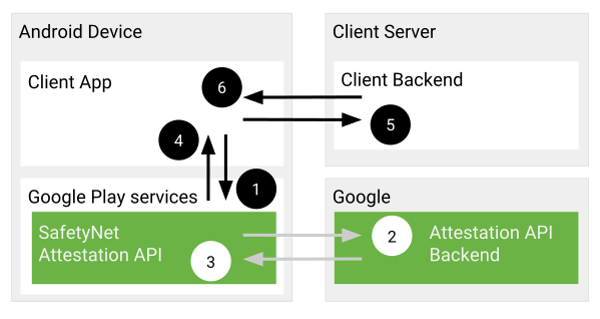
\includegraphics[width=0.7\textwidth]{img/safetynet_attestation}
	\caption{SafetyNet Attestation API protocol~\cite{safetynet_attestation}.}
	\label{fig:safetynet_attestation}
\end{figure}
\end{frame}

% \begin{frame}{SafetyNet: Attestation response}
% Two important parameters:
% \begin{description}
%   \item[ctsProfileMatch] Device matches the profile of a device that has passed the compatibility test
%   \item[basicIntegrity] Device was not tampered with but has not necessarily passed the compatibility test
% \end{description}
% \end{frame}



\begin{frame}{SafetyNet: Attestation results}
\begin{table}
  \begin{tabular}{l | c | c }

      \textbf{Device Status} & \textbf{Value of} &  \textbf{Value of}\\
       & \textbf{ctsProfileMatch} & \textbf{basicIntegrity}\\
      \hline
       Certified, genuine device that passes CTS & true &true\\
       Certified device with unlocked bootloader&false&true\\
       Genuine but uncertified device &false&true\\
       Device with custom ROM (not rooted)&false&true\\
       Emulator&false &false \\
       No device (protocol emulator script) &false &false \\
       Signs of system integrity compromise (rooting) &false &false \\
       Signs of other active attacks (API hooking) &false &false \\

  \end{tabular}
  \caption{Possible SafetyNet Attestation results~\cite{safetynet_attestation}.}
  \label{table:safetynet_attestation_results}
\end{table}
\end{frame}


%%%%%%%%%%%%%%%%%%%%%%%%%%%%%%%%%%%%%%%%%%%%%%%%%%%%%
\begin{frame}{Verified Boot}
\begin{itemize}
  \item Guarantees integrity of the device software from the bootloader up to the operating system\newline
  \item Partitions are divided into 4 KiB blocks, which are verified against a signed hash tree when read\newline
  \item It is not possible anymore to roll back to an earlier OS version\newline
  \item Bootloader can only be unlocked by a user physically interacting with it

\end{itemize}
\begin{description}
  \item[Device state] Locked or unlocked bootloader
  \item[Boot state] Indicates the state of device integrity

\end{description}
\end{frame}

% \begin{frame}{Verified Boot}
% \begin{figure}[t]
% 	\centering
% 	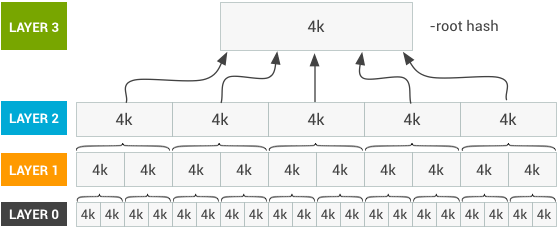
\includegraphics[width=0.7\textwidth]{img/dm-verity-hash-table}
% 	\caption{dm-verity hash tree~\cite{android_verified_boot}.}
% 	\label{fig:dm-verity-hash-table}
% \end{figure}
% \end{frame}


\begin{frame}{Verified Boot: boot states}
\begin{figure}[t]
	\centering
	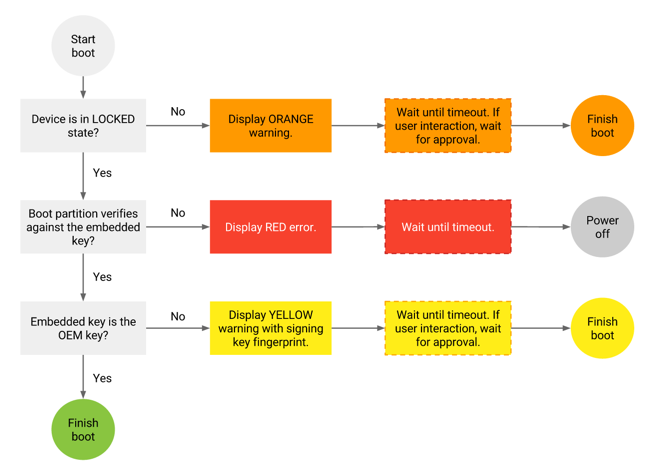
\includegraphics[width=0.65\textwidth]{img/verified_boot}
	\caption{Verified boot flow~\cite{android_verified_boot}.}
	\label{fig:android_verified_boot}
\end{figure}
\end{frame}





%%%%%%%%%%%%%%%%%%%%%%%%%%%%%%%%%%%%%%%%%%%%%%%%%%%%%
\begin{frame}{Updates}
\begin{itemize}
  \item Diverse and sometimes short update period device manufacturers provide\newline
  --> Popularity of custom ROMs\newline
  \item New approach by Google:\newline
  -Linux LTS kernels switch from 2 year to 6 year life cicle of support\newline
  -\alert{Project Treble} since Android 8\newline
  \end{itemize}
  -->  Separation of Android OS and vendor implementation\newline\newline
  -->  Faster, easier and less expensive update process

\end{frame}


% \begin{frame}{Updates: Project Treble}
% \begin{figure}[H]
% 	\centering
% 	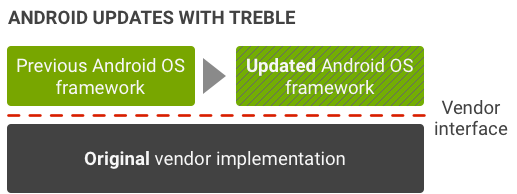
\includegraphics[width=0.7\textwidth]{img/treble_after.png}
% 	\caption{The new update process with Project Treble~\cite{android_treble}.}
% 	\label{fig:project_treble}
% \end{figure}
% \end{frame}


%%%%%%%%%%%%%%%%%%%%%%%%%%%%%%%%%%%%%%%%%%%%%%%%%%%%%
\begin{frame}{Rooting: soft root vs. hard root}

\begin{exampleblock}{Soft root}
\begin{itemize}
  \item Exploiting security \alert{vulnerabilities}
  \item Device vulnerable to malware
  \item Only option for devices with unlockable bootloader
\end{itemize}
\end{exampleblock}
\begin{exampleblock}{Hard root}
\begin{itemize}
  \item \alert{Su} binary is flashed through a custom recovery
  \item or included in a custom ROM
  \item Systemless-ly approach: \alert{system} partition untouched
\end{itemize}
\end{exampleblock}

\end{frame}





%%%%%%%%%%%%%%%%%%%%%%%%%%%%%%%%%%%%%%%%%%%%%%%%%%%%%
%
%
%%%%%%%%%%%%%%%%%%%%%%%%%%%%%%%%%%%%%%%%%%%%%%%%%%%%
\section{LineageOS}

\begin{frame}{LineageOS}
	\begin{itemize}
    \item Over 1.87 million active installations on 180 different devices\newline
    \item Patches several security vulnerabilities, which are not be addresses anymore by OEMs\newline
    \item Device requirements, which must be met for a device to be ready to receive a LineageOS release\newline
    \item Provides su addon
  \end{itemize}
\end{frame}

\begin{frame}{LineageOS: applications}
\begin{itemize}
  \item Own unique apps not found in AOSP\newline
  \item Comes without Google apps, but can be flashed\newline
  \item Apps have to be installed manually by the user\newline
  \item Alternative app store e.g. F-Droid for FOSS apps
\end{itemize}
\end{frame}


\begin{frame}{LineageOS: Privacy Guard}
\begin{itemize}
  \item Permission manager of applications\newline
  \item Seetings can be adjusted fine grained\newline
  \item Manages root access
\end{itemize}
\end{frame}


\begin{frame}{LineageOS: su addon}
\begin{itemize}
  \item Separate su addon package\newline
  \item Su binary in \emph{/system/xbin}\newline
  \item Su can be turned on/off in settings (default: off)\newline
\end{itemize}
\end{frame}


\begin{frame}{LineageOS: su request}
\begin{figure}
  \centering
  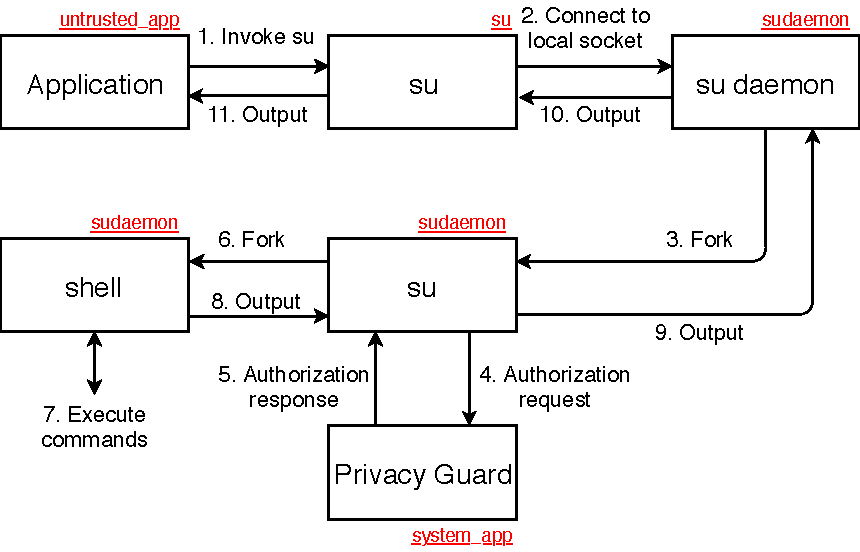
\includegraphics[width=0.7\textwidth]{img/lineage_su}
  \caption{Procedure diagram of invoking su by an application.}
  \label{fig:lineage_procedure_su_call}
\end{figure}
\end{frame}



\begin{frame}{LineageOS: security implications}
\begin{itemize}
  \item Unlocked bootloader, no Verified Boot (Recowvery, CVE-2016-5195)\newline
  --> No hardware based root of trust
  \item Manual installation of apps
\end{itemize}
\begin{exampleblock}{Attack possibilities against}
\begin{itemize}
  \item Su and su daemon (CVE-2013-6768, -6769, -6770, -6774, -6775)
  \item local socket file (0666 permission, /dev/socket/su-daemon/)
  \item Privacy Guard
\end{itemize}
\end{exampleblock}
\begin{itemize}
  \item SELinux for su and su daemon in permissive mode
\end{itemize}
\end{frame}

% \begin{frame}{LineageOS: security implications}
%    Unlocked bootloader, no Verified Boot, no hardware based root of trust
%    \begin{itemize}
%    \item Revowvery: flashing recovery on secure systems with unlocked bootloaders
%    (Dirty Cow, CVE-2016-5195)
% \end{itemize}
% \textbf{SU and SU daemon}
%    \begin{itemize}
%   \item PATH not properly set: manipulation of environment variables and file descriptors (CVE-2013-6768)
%   \item Manipulation of \emph{bootclasspath} allowed loading arbitrary .jar file and gain root privileges (CVE-2013-6774)
%   \item Trick forked root shell to run arbitrary commands although SU request was denied by user (CVE-2013-6769, CVE-2013-6775)
%   \item Ability to restart SU daemon and execut malicious app (ADB Shell access, granted root permission before, special UID) (CVE-2013-6770)
% \end{itemize}
% \end{frame}

%
% \begin{frame}{LineageOS: security implications}
% \begin{itemize}
%   \item Local socket file
%   \item Privacy Guard
% \end{itemize}
% \end{frame}





\begin{frame}{LineageOS: evaluation}
\textbf{Application behaviour}
\begin{enumerate}
\item LineageOS unmodified\newline
--> Apps not working (due to missing Google Services)\newline
\item LineageOS with su addon\newline
--> Apps not working (due to missing Google Services)\newline
\item LineageOS with GApps (OpenGApps, \emph{pico} and \emph{stock} version)\newline
--> Apps working when installed via Google Play\newline
\item LineageOS with GApps and \emph{su} addon\newline
--> Apps working when su addon turned off\newline

\end{enumerate}
\end{frame}


\begin{frame}[fragile]{LineageOS: evaluation}
\textbf{SafetyNet}

\begin{minted}[mathescape,gobble=0,frame=lines,fontsize=\footnotesize]{bash}
# disabled root access
SafetyNetResponse: ...
"ctsProfileMatch":false,
"basicIntegrity":true,
"advice":"RESTORE\_TO\_FACTORY\_ROM,LOCK\_BOOTLOADER"

# enabled root access
SafetyNetResponse: ...
"ctsProfileMatch":false,
"basicIntegrity":false,
"advice":"RESTORE\_TO\_FACTORY\_ROM,LOCK\_BOOTLOADER"
\end{minted}
\end{frame}



%%%%%%%%%%%%%%%%%%%%%%%%%%%%%%%%%%%%%%%%%%%%%%%%%%%%%
%
%
%%%%%%%%%%%%%%%%%%%%%%%%%%%%%%%%%%%%%%%%%%%%%%%%%%%%
\section{Magisk}

\begin{frame}{Magisk}
\begin{itemize}
  \item Set of tools, which establish an environment to alter Android \alert{systemless-ly}\newline
  \item Accomplished by only patching the boot image\newline
  \item Can hide modifications from system integrity verifications like Safety\newline
  \item Provides rooting solution MagiskSU
\end{itemize}
\end{frame}

\begin{frame}[fragile]{Magisk: initialization}
\begin{itemize}
  \item Init is replaced with MagiskInit and executed afterwards\newline
  \item Adds own init.Magisk.rc file to init.rc\newline
  \item Starts services: Magisk daemon, MagiskHide\newline
  \item SELinux policy file is patched\newline
  \item Files reside in /root with symlinks in /sbin (tmpfs)
\end{itemize}

% \begin{minted}[mathescape,gobble=0,frame=lines,fontsize=\footnotesize]{bash}
% magiskboot                   /* binary */
% magiskinit                   /* binary */
% magiskpolicy -> magiskinit
% supolicy -> magiskinit       /* alias of magiskpolicy */
% magisk                       /* binary */
% magiskhide -> magisk
% resetprop -> magisk
% su -> magisk
% \end{minted}
\end{frame}




% \begin{frame}[fragile]{Magisk: initialization}
% Excerpts of the /sbin folder
% \begin{minted}[mathescape,gobble=0,frame=lines,fontsize=\footnotesize]{bash}
% lrwxrwxrwx  1 root root  magisk       -> /root/WsfdiYsya
% lrwxrwxrwx  1 root root  magiskhide   -> /root/WsfdiYsya
% lrwxrwxrwx  1 root root  magiskpolicy -> /root/tg3PvPmOx
% lrwxrwxrwx  1 root root  resetprop    -> /root/WsfdiYsya
% lrwxrwxrwx  1 root root  su           -> /root/WsfdiYsya
% lrwxrwxrwx  1 root root  supolicy     -> /root/tg3PvPmOx
% \end{minted}
% \end{frame}



\begin{frame}{MagiskSU}
\begin{figure}
	\centering
	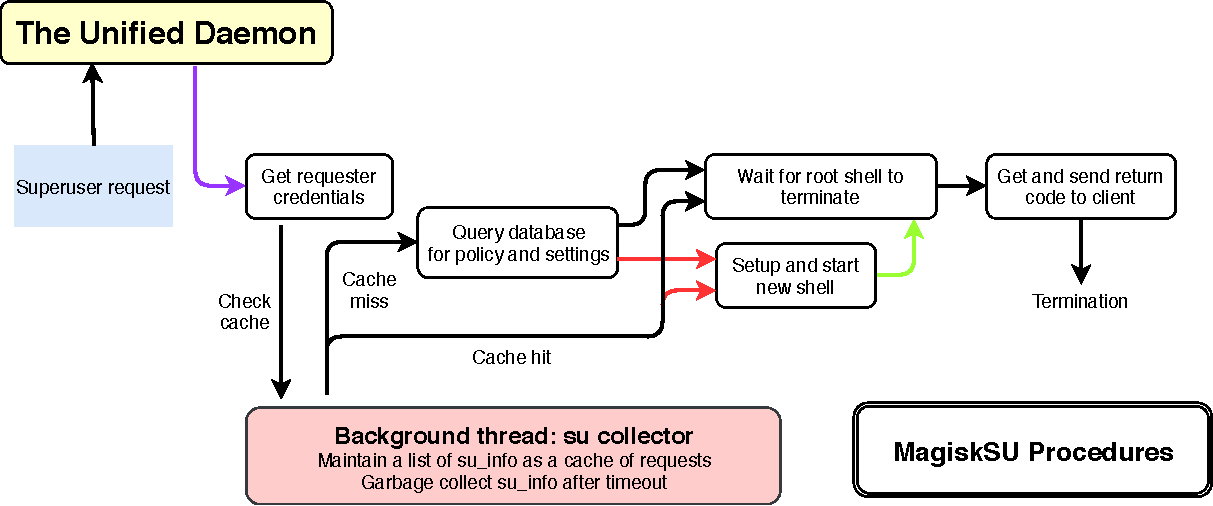
\includegraphics[width=0.9\textwidth]{img/magisk_su_procedures}
	\caption{Procedure diagram of invoking su by an application~\cite{magisk_documentation}.}
	\label{fig:magisk_su_procedures_diagram}
\end{figure}
\end{frame}


\begin{frame}{MagiskSU <--> LineageOS su}
They share the same su code base\newline
\begin{itemize}
  \item Su collector as cache\newline
  \item Su SELinux label (u:r:su:s0) <--> su and sudaemon label\newline

  \item Magisk Manager <--> Privacy Guard\newline
  \item Broadcast request intent <--> AppOpsManager API
\end{itemize}
\end{frame}






\begin{frame}{Magisk: security implications}
\begin{itemize}
  \item Unlocked bootloader, no Verified Boot (Recowvery, CVE-2016-5195)\newline
  --> No hardware based root of trust
\end{itemize}
\begin{exampleblock}{Attack possibilities against}
\begin{itemize}
  \item Su and su daemon (CVE-2013-6768, -6769, -6770, -6774, -6775)
  \item local socket file (0777 permission, /dev/.socketXXXXX)
  \item Su request intent
  \item policy database
\end{itemize}
\end{exampleblock}
\begin{itemize}
  \item SELinux for su in permissive mode
  \item New SELinux policies for su
\end{itemize}
\end{frame}


\begin{frame}{MagiskHide}
Hides Magisk, Magisk Manager or an unlocked bootloader from apps or system integrity checks
\begin{itemize}
\item Keeps a list of apps to hide from (managed in Magisk Manager)\newline
\item Monitors Logcat \alert{am\_proc\_start} events\newline
\item Target will be paused immediately (SIGSTOP), new process is forked\newline
\item Process joins mount namespace and hides sensitive properties\newline
\item \emph{tmpfs} /sbin is unmounted\newline
\item Target is allowed to continue (SIGCONT)
\end{itemize}
\end{frame}





\begin{frame}[fragile]{MagiskHide: sensitive properties}
\begin{minted}[mathescape,linenos,gobble=0,frame=lines,fontsize=\footnotesize]{bash}
ro.boot.verifiedbootstate  = green
ro.boot.flash.locked       = 1
ro.boot.veritymode         = enforcing
ro.boot.warranty_bit       = 0
ro.warranty_bit            = 0
ro.debuggable              = 0
ro.secure                  = 1
ro.build.type              = user
ro.build.tags              = release-keys
ro.build.selinux           = 0
\end{minted}
\end{frame}




\begin{frame}{Magisk: evaluation}
\textbf{Application behaviour}
\begin{exampleblock}{MagiskHide enabled}
\begin{itemize}
  \item Most applications work
  \item Some check the installed packages and recognize Magisk Manager
  \item \alert{Solution}: Hide Magisk Manger with random package name
\end{itemize}
\end{exampleblock}
\begin{exampleblock}{MagiskHide disabled}
\begin{itemize}
  \item Most applications do not work
  \item \alert{Error message}: device does not have the necessary safety mechanisms or device is rooted
\end{itemize}
\end{exampleblock}
\end{frame}







\begin{frame}[fragile]{Magisk: evaluation}
\textbf{SafetyNet}
\begin{minted}[mathescape,gobble=0,frame=lines,fontsize=\footnotesize]{bash}
# MagiskHide disabled
SafetyNetResponse: ...
"ctsProfileMatch":false,
"basicIntegrity":false,
"advice":"RESTORE\_TO\_FACTORY\_ROM"

# MagiskHide enabled
SafetyNetResponse: ...
"ctsProfileMatch":true,
"basicIntegrity":true
\end{minted}
\end{frame}


%%%%%%%%%%%%%%%%%%%%%%%%%%%%%%%%%%%%%%%%%%%%%%%%%%%%%
%
%
%%%%%%%%%%%%%%%%%%%%%%%%%%%%%%%%%%%%%%%%%%%%%%%%%%%%
\section{Root detection}

\begin{frame}{Root detection methods}
How detect apps if a device is rooted?
  \begin{enumerate}
    \item Presence of files
    \item System properties
    \item Directory permissions
    \item Installed packages
    \item Processes, Services and Tasks
    \item Shell commands
  \end{enumerate}
\end{frame}


\begin{frame}{Root detection: presence of files}
\begin{itemize}
  \item Check existence of files in certain direcories

  /system/xbin, /system/bin, /system/app, /sbin, /data/app\newline
  \item Parsing \emph{PATH} and appending \emph{/su} to each entry
  \item Using \emph{which} combined with \emph{su}
\end{itemize}
\end{frame}


\begin{frame}{Root detection: system properties}
Check certain entries in \alert{/system/build.prop} using \emph{getprop}
\begin{exampleblock}{Queried entries}
\begin{itemize}
  \item \emph{ro.build.tags =release-keys}
  \item \emph{ro.build.type = user}
  \item \emph{ro.debuggable = 0}
  \item \emph{ro.secure = 1}
\end{itemize}
\end{exampleblock}
\end{frame}



\begin{frame}{Root detection: directory permissions}
Check directory permissions using common functions and the Java API
\begin{exampleblock}{Used functions}
\begin{itemize}
  \item \emph{access(3P)}
  \item \emph{canRead()}
  \item \emph{canWrite()}
\end{itemize}
\end{exampleblock}
\end{frame}


\begin{frame}{Root detection: installed packages}
Use \alert{PackageManger} API to retrieve installed packages
\begin{exampleblock}{Used functions}
\begin{itemize}
  \item \emph{getInstalledPackages()}
  \item \emph{getInstalledApplications()}
  \item \emph{pm list packages}
\end{itemize}
\end{exampleblock}
\end{frame}



\begin{frame}{Root detection: processes, services and tasks}
Use \alert{ActivityManager} API to retrieve information about proccesses, services and tasks
\begin{exampleblock}{Used functions}
\begin{itemize}
  \item \emph{get.RunningAppProcesses()}
  \item \emph{get.Running.Services()}
  \item \emph{get.RecentTasks()}
\end{itemize}
\end{exampleblock}
\end{frame}




\begin{frame}{Root detection: shell commands}
Use common shell commands to retrieve information on files and folders
\begin{exampleblock}{Used functions}
\begin{itemize}
  \item \emph{ls}
  \item \emph{ps | grep <name>}
  \item \emph{pm path <packagename>}
\end{itemize}
\end{exampleblock}
\end{frame}





%%%%%%%%%%%%%%%%%%%%%%%%%%%%%%%%%%%%%%%%%%%%%%%%%%%%%
%
%
%%%%%%%%%%%%%%%%%%%%%%%%%%%%%%%%%%%%%%%%%%%%%%%%%%%%
\section{Jailbreaking iOS}
\begin{frame}{Jailbreaking iOS}
\begin{itemize}
  \item Closed source operating system with software restrictions
  \item Jailbreaking <-> exploiting \alert{security vulnerabilities}
  \item Not available for every iOS versions
  \item Best compared to \alert{soft rooting} Android
\end{itemize}
Not recommended for devices handling \alert{sensitive information} since attackers can use vulneratiblities, too!
\end{frame}







%%%%%%%%%%%%%%%%%%%%%%%%%%%%%%%%%%%%%%%%%%%%%%%%%%%%%
%
%
%%%%%%%%%%%%%%%%%%%%%%%%%%%%%%%%%%%%%%%%%%%%%%%%%%%%
\section{Conclusion}

\begin{frame}{Summary}
\begin{itemize}
  \item There are opportunities for attacks, but no current known attacks\newline
  --> no less secure than other software\newline
  \item no Verified Boot\newline
  \item Root detection: No distinction hard <-> soft root\newline
  --> No justification for excluding such devices from certain apps.\newline
  \item Security relies on user and his decisions\newline
  \item Custom ROMs often the only possibility to get updates\newline
  \item Cat and mouse game between Google and the rooting community\newline

\end{itemize}
\end{frame}















%%%%%%%%%%%%%%%%%%%%%%%%%%%%%%%%%%%%%%%%%%%%%%%%%%%%%
%
%
%%%%%%%%%%%%%%%%%%%%%%%%%%%%%%%%%%%%%%%%%%%%%%%%%%%%
\begin{frame}[standout]
  Questions?
\end{frame}



\appendix




\begin{frame}[fragile]{SELinux}
\begin{figure}[H]
  \centering
  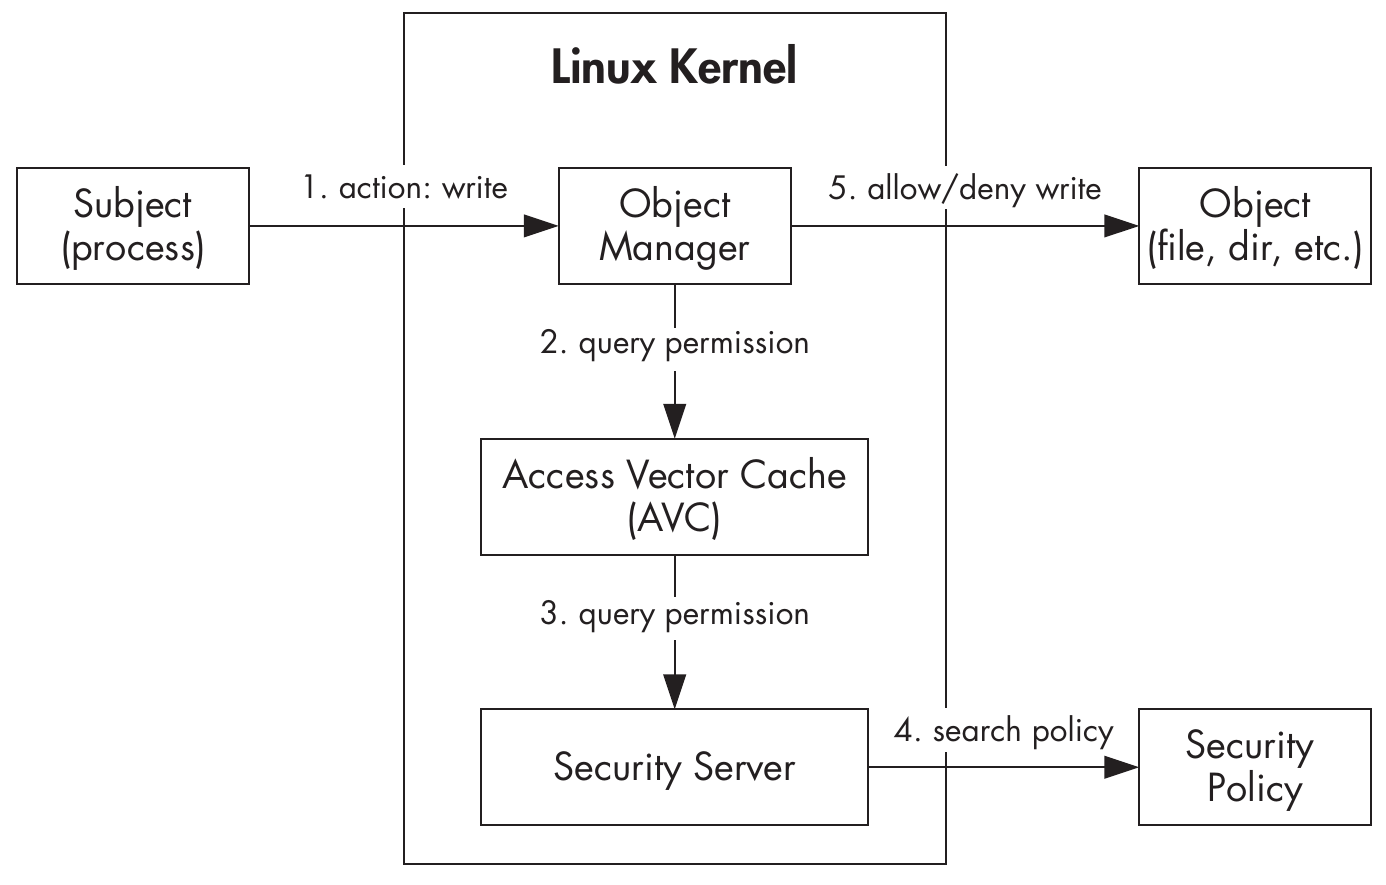
\includegraphics[width=0.7\textwidth]{img/selinux}
  \caption{SELinux components~\cite{android_sec_internals}.}
  \label{fig:selinux}
\end{figure}
\end{frame}



\begin{frame}[fragile]{SafetyNet: Attestation payload}
\begin{minted}[mathescape,gobble=0,linenos,frame=lines,fontsize=\footnotesize]{bash}
  "nonce": "R2Rra24fVm5xa2Mg",
  "timestampMs": 9860437986543,
  "apkPackageName": "com.package.name.of.requesting.app",
  "apkCertificateDigestSha256": ["base64 encoded, SHA-256 hash of the
                                  certificate used to sign requesting app"],
  "apkDigestSha256": ["base64 encoded, SHA-256 hash of
                      the APK installed on a user's device"],
  "ctsProfileMatch": true,
  "basicIntegrity": true,
\end{minted}
\end{frame}



\begin{frame}{SafetyNet: additional APIs}
\begin{description}
  \item[Safe Browsing API] determines if an URL has been marked as a known threat
  \item[reCAPTCHA API] uses reCAPTCHA to protect apps from malicious traffic/spam
  \item[Verify Apps API] protects devices against potentially harmful apps
\end{description}
\end{frame}




\begin{frame}{Verified Boot: hash tree}
\begin{figure}[t]
	\centering
	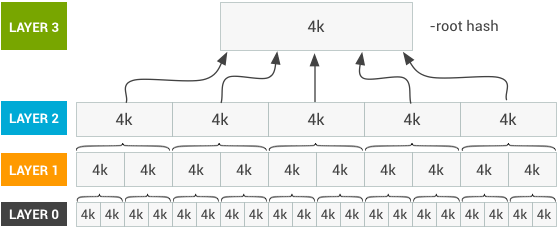
\includegraphics[width=0.9\textwidth]{img/dm-verity-hash-table}
	\caption{dm-verity hash tree~\cite{android_verified_boot}.}
	\label{fig:dm-verity-hash-table}
\end{figure}
\end{frame}




\begin{frame}{Updates: Project Treble }
\begin{figure}[H]
	\centering
	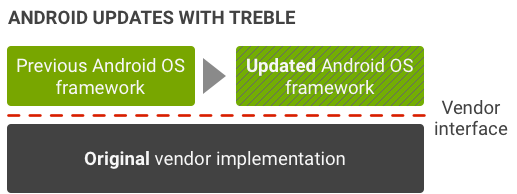
\includegraphics[width=0.7\textwidth]{img/treble_after.png}
	\caption{The update process before Project Treble~\cite{android_treble}.}
	\label{fig:project_treble}
\end{figure}
\end{frame}



\begin{frame}[fragile]{LineageOS: shell escape vulnerability}
\begin{minted}[mathescape,gobble=0,linenos,frame=lines,fontsize=\footnotesize]{bash}
"su -c 'COMMAND' "

...
ctx->from.uid, ctx->to.uid, get_command(&ctx->to),
policy == ALLOW ? "allow" : "deny", ctx->user.android_user_id);


get_command() would return "COMMAND", unescaped

su -c "'&touch /data/test;'"
su -c '`touch /data/test`'
su -c '$(touch /data/test)'
\end{minted}
\end{frame}




\begin{frame}{MagiskHide: procedure diagram}
\begin{figure}
	\centering
	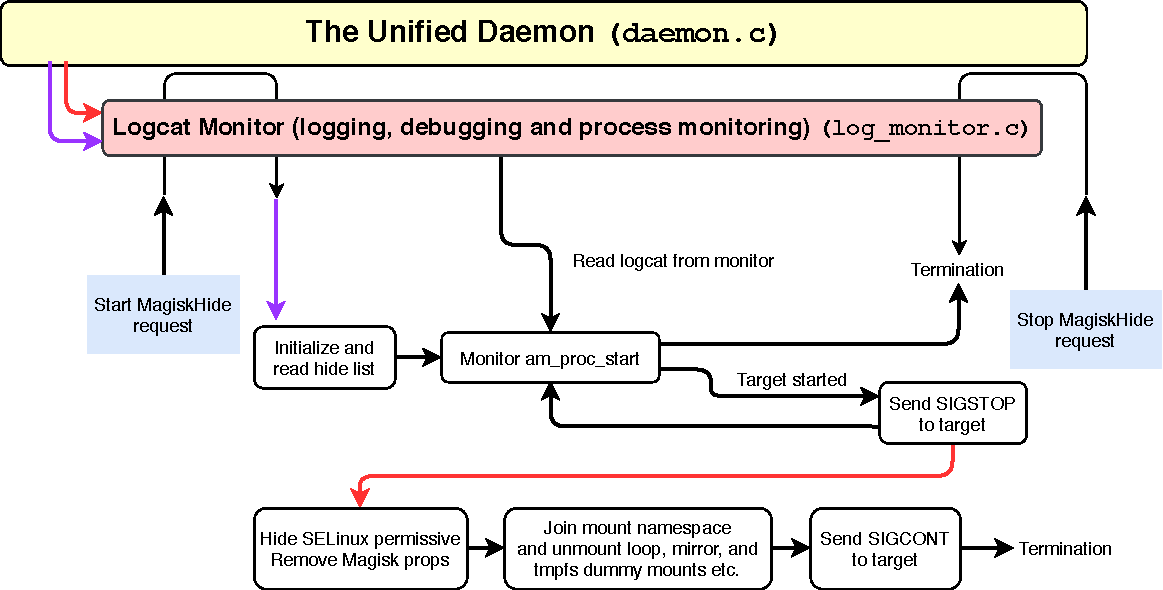
\includegraphics[width=0.9\textwidth]{img/magisk_hide}
	\caption{Procedure diagram of MagiskHide~\cite{magisk_documentation}.}
	\label{fig:magisk_hide}
\end{figure}
\end{frame}


\begin{frame}[fragile]{Magisk: Magisk tools}
\begin{minted}[mathescape,linenos,gobble=0,frame=lines]{bash}
magiskboot                 /* binary */
magiskinit                 /* binary */
magiskpolicy -> magiskinit
supolicy -> magiskinit     /* alias of magiskpolicy */
magisk                     /* binary */
magiskhide -> magisk
resetprop -> magisk
su -> magisk
\end{minted}
\end{frame}


\begin{frame}[fragile]{Magisk: structure I}
\begin{minted}[mathescape,gobble=0,frame=lines]{c}
LOGFILE         "/cache/magisk.log"
DISABLEFILE     "/cache/.disable_magisk"
UNINSTALLER     "/cache/magisk_uninstaller.sh"
CACHEMOUNT      "/cache/magisk_mount"
MAINIMG         "/data/adb/magisk.img"
DATABIN         "/data/adb/magisk"
MANAGERAPK      "/data/adb/magisk/magisk.apk"
DEBUG_LOG       "/data/adb/magisk_debug.log"
UNBLOCKFILE     "/dev/.magisk.unblock"
PATCHDONE       "/dev/.magisk.patch.done"
MAGISKRC        "/init.magisk.rc"
MAGISKTMP       "/sbin/.core"
MIRRDIR         "/sbin/.core/mirror"
BBPATH          "/sbin/.core/busybox"
MOUNTPOINT      "/sbin/.core/img"
COREDIR         "/sbin/.core/img/.core"
HOSTSFILE       "/sbin/.core/img/.core/hosts"
HIDELIST        "/sbin/.core/img/.core/hidelist"
\end{minted}
\end{frame}


\begin{frame}[fragile]{Magisk: structure II}
\begin{minted}[mathescape,gobble=0,frame=lines]{c}
BBPATH          "/sbin/.core/busybox"
MOUNTPOINT      "/sbin/.core/img"
COREDIR         "/sbin/.core/img/.core"
HOSTSFILE       "/sbin/.core/img/.core/hosts"
HIDELIST        "/sbin/.core/img/.core/hidelist"
\end{minted}
\end{frame}

\begin{frame}{Magisk: resetprop}
\begin{itemize}
  \item created by pulling out the portion of source code managing properties from AOSP
  \item try to mimic what init is doing.
  \item Result: direct access to the data structure
  \item Property deletion is accomplished by detaching the target node from the tree structure, making it effectively invisible.
\end{itemize}
\end{frame}



\begin{frame}[fragile]{Analyzed applications}
\begin{exampleblock}{Banking}
\begin{itemize}
\item Sparkasse, Sparkasse pushTAN
\item VR-Banking, VR-SecureGo
\item DKB-Banking, DKB-TAN2go
\item Deutsche Bank Mobile
\item ING-DiBa Banking to go, ING-DiBa Banking + Brokerage
\item o2 Banking, Commerzbank Banking, N26
\end{itemize}
\end{exampleblock}
\begin{exampleblock}{Antivirus, Root checker}
\begin{itemize}
\item Avira, Kaspersky, Avast, McAfee, Eset Mobile Security, AVG Mobile
\item Root Checker (3x), Root Check
\end{itemize}
\end{exampleblock}
\end{frame}



\begin{frame}[allowframebreaks]{References}

  \bibliography{references}
  \bibliographystyle{abbrv}

\end{frame}

\end{document}
